\subsubsection{Komponen \textbf{\textit{Flexible Control}}}
\textbf{\textit{Flexible Control}} akan mengkolaborasikan \textbf{\textit{Rule Manager}}, \textbf{\textit{Resource Controller}}, \textbf{\textit{Predict Component Factory}} dan \textbf{\textit{Predict Component Storage}}. Komponen ini akan meminta list waktu prediksi yang diperlukan dari \textbf{\textit{Rule Manager}} untuk \textbf{\textit{Rule Manager}} sehingga \textbf{\textit{Predict Component Storage}} dapat menyediakan data prediksi. Setelah itu, semua \textbf{\textit{Rule}} yang memenuhi syarat akan langsung ditransformasikan dan dikirim ke komponen \textbf{\textit{Resource Controller}}. Selain itu, komponen ini juga bertanggung jawab meneruskan data ke \textbf{\textit{Predict Component Storage}} untuk melakukan penambahan data. Spesifikasi kelas ini dapat dilihat pada gambar \ref{fig:ac-spek}.

\begin{figure}[h]
    \centering
    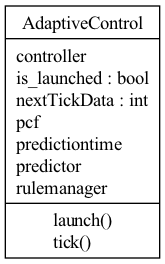
\includegraphics[width=0.3\textwidth]{chapter-4/ac.png}
    \caption{Spesifikasi Kelas Penyusun Komponen \textit{Flexible Control}}
    \label{fig:ac-spek}
\end{figure}